\documentclass[12pt]{article}

% -----------------------------------------------------------------------
% Packages
% -----------------------------------------------------------------------
\usepackage[margin=1in]{geometry}
\usepackage{setspace}
\doublespacing
\usepackage{amsmath, amssymb}
\usepackage{booktabs}
\usepackage{graphicx}
\usepackage{float}
\usepackage{caption}
\usepackage{subcaption}

% Required by modelsummary (tabularray output)
\usepackage{tabularray}
\usepackage{codehigh}
\usepackage[normalem]{ulem}
\UseTblrLibrary{booktabs}
% siunitx not available in this TeX installation; stub out \num
\providecommand{\num}[1]{#1}
\newcommand{\tinytableTabularrayUnderline}[1]{\underline{#1}}
\newcommand{\tinytableTabularrayStrikeout}[1]{\sout{#1}}
\NewTableCommand{\tinytableDefineColor}[3]{\definecolor{#1}{#2}{#3}}
\usepackage{hyperref}
\hypersetup{colorlinks=true, linkcolor=black, citecolor=black, urlcolor=blue}

% Bibliography – using natbib + bibtex (biblatex not available in this env)
\usepackage[authoryear,round,comma,sort]{natbib}

% Tables
\usepackage{threeparttable}
\usepackage{pdflscape}

% -----------------------------------------------------------------------
% Title
% -----------------------------------------------------------------------
\title{Firm Entry and AI:\\
       Evidence from the US}
\author{Guillermo Gallacher%
       \thanks{Indeed Hiring Lab and Universidad del CEMA. \href{mailto:guillermogallacher@gmail.com}{guillermogallacher@gmail.com}}}
\date{\today \\ \medskip \small Preliminary and incomplete. Comments welcome.}

% -----------------------------------------------------------------------
\begin{document}
% -----------------------------------------------------------------------

\maketitle

\begin{abstract}
  \noindent
  [Abstract placeholder. Summarise: motivation, data, method, main finding,
  contribution. Roughly 150--200 words.]
\end{abstract}

\noindent\textbf{Keywords:} business formation, artificial intelligence,
  AI exposure, difference-in-differences, ChatGPT

\noindent\textbf{JEL codes:} L26, O33, J24, M13

\clearpage

% -----------------------------------------------------------------------
\section{Introduction}
\label{sec:intro}
% -----------------------------------------------------------------------

The arrival of large language models---most visibly the public release of
ChatGPT in November 2022---has revived interest in how general-purpose
technologies reshape labour markets and firm dynamics
\citep{felten2021occupational, fossen2024new}.
Most of this debate focuses on \emph{workers}: which jobs are at risk, and
for whom.
But a parallel question may be equally consequential: does AI alter the
incentives to \emph{start} a business?

\begin{figure}[H]
  \centering
  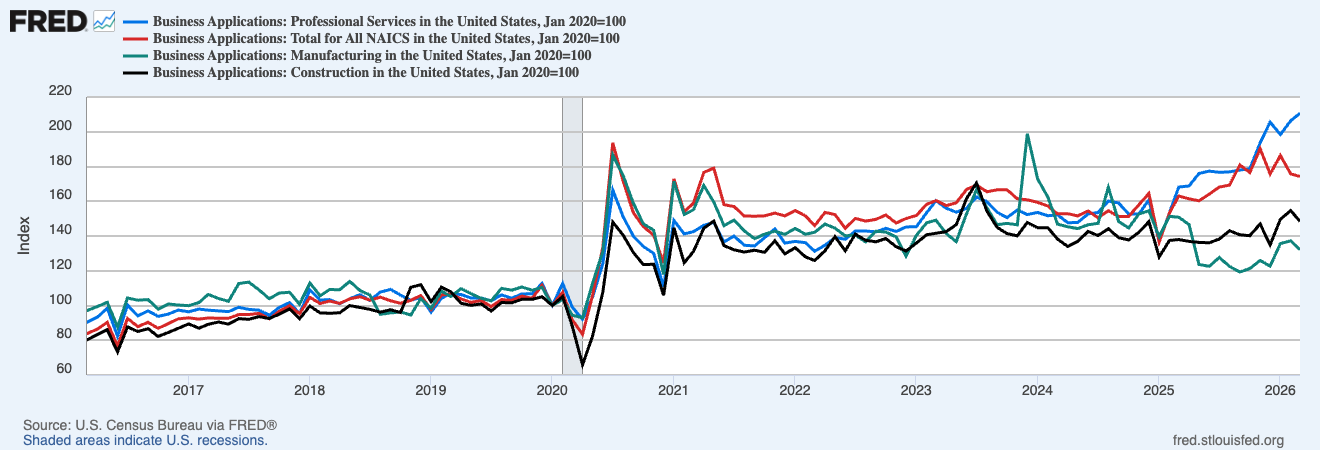
\includegraphics[width=0.88\textwidth]{fig_fred_motivation}
  \caption{Business applications indexed to January 2020~$=100$ for selected
           sectors. Source: U.S.\ Census Bureau via FRED
           (\url{https://fred.stlouisfed.org/graph/?g=1UHD5}).
           Shaded area indicates the COVID-19 recession (Feb--Apr 2020).}
  \label{fig:fred}
\end{figure}

Figure~\ref{fig:fred} offers a first look.
After the COVID-19 shock, aggregate business applications surged to historic
highs and have continued rising through 2025.
But the expansion is not uniform.
Professional and Business Services---among the most AI-exposed sectors by
any measure---have pulled sharply away from the aggregate trend.
Manufacturing and Construction, where tasks are less amenable to
language-model automation, have lagged behind.
This heterogeneity motivates the present paper.

Lower entry costs, improved productivity for high-skilled tasks, and
easier access to specialised knowledge may all reduce barriers to
entrepreneurship in AI-exposed sectors \citep{brynjolfsson2018can}.
Conversely, if AI primarily benefits large incumbents, competitive pressures
could \emph{raise} barriers to entry.
Distinguishing between these channels requires variation both across sectors
and over time---variation the public release of ChatGPT conveniently provides.

We use monthly sector-level business application counts from the Census Bureau
Business Formation Statistics \citep{haltiwanger2020bfs} together with the
AI Industry Exposure (AIIE) index of
\citeauthor{felten2021occupational}~(\citeyear{felten2021occupational})
to estimate a difference-in-differences (DiD) model of the form
\begin{equation}
  \log(\text{BA}_{it}) \;=\; \alpha_i + \gamma_t
    + \beta\,(\text{Post}_t \times \text{AI Exposure}_i) + \varepsilon_{it},
  \label{eq:did}
\end{equation}
where $\text{Post}_t$ is an indicator equal to one from November 2022 onwards,
$\alpha_i$ are sector fixed effects absorbing time-invariant differences in
application rates, and $\gamma_t$ are month fixed effects absorbing aggregate
cyclical variation.
The coefficient $\beta$ identifies whether sectors with higher AI exposure
experienced a differential change in business formation after ChatGPT.



\paragraph{Related literature.}
\citet{fossen2024new} examine AI adoption and self-employment at the
individual level and find positive effects concentrated among high-skilled
workers.
\citet{felten2021occupational} construct the AIOE/AIIE index by combining
O*NET task measures with AI capability scores.
\citet{haltiwanger2020bfs} describe the Census Bureau BFS and demonstrate
its value for studying business dynamism and entry margins.
\citet{brynjolfsson2018can} provide a conceptual framework for mapping
task-level AI capabilities to occupational and industry outcomes.

% -----------------------------------------------------------------------
\section{Data}
\label{sec:data}
% -----------------------------------------------------------------------

\subsection{Business Formation Statistics}
\label{sec:data_bfs}

The Census Bureau BFS provides monthly, seasonally adjusted counts of new
Employer Identification Number (EIN) applications at the 2-digit NAICS
level, derived from IRS Form~SS-4 filings \citep{haltiwanger2020bfs}.
EIN applications are a leading indicator of actual business formation:
roughly half of high-propensity applicants open within eight quarters of
filing.
We use the official seasonally adjusted series directly and index each
sector to January 2020~$= 100$, yielding a panel of 20 sectors observed
from January 2006 through early~2026.
We define two treatment dates: November~2022 (public launch of ChatGPT)
and May~2025 (widespread availability of agentic AI tools).

Figure~\ref{fig:spotlight} plots the index for four selected sectors.
The divergence between Professional Services and goods-producing sectors
is visible from approximately 2021 and widens after November 2022,
consistent with a role for AI in lowering barriers to entry specifically
where tasks are more cognitively intensive.

\begin{figure}[H]
  \centering
  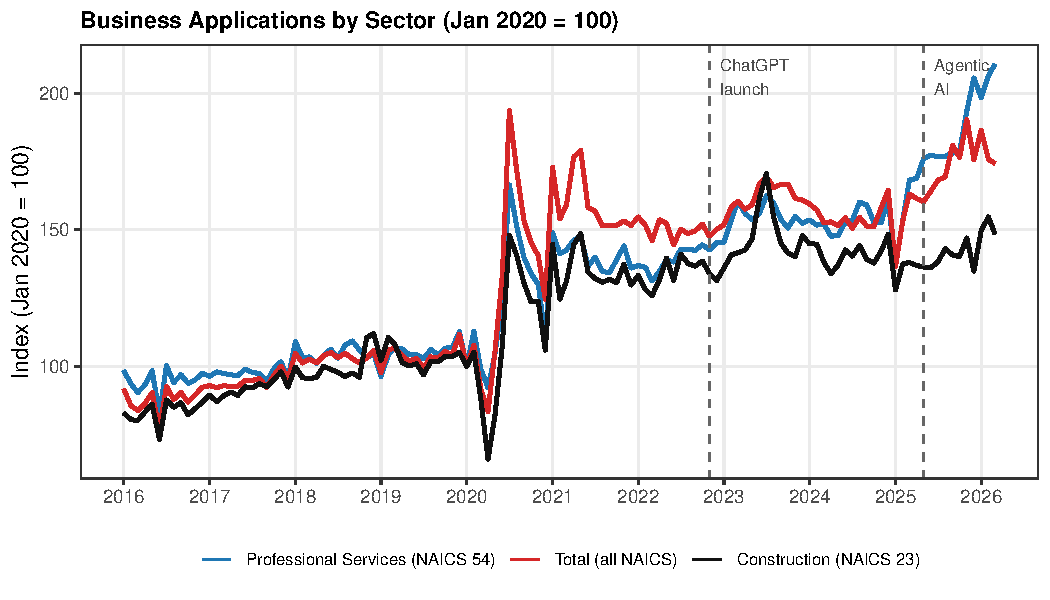
\includegraphics[width=0.88\textwidth]{fig_spotlight}
  \caption{Business applications indexed to January 2020~$=100$.
           Professional Services (NAICS~54), Total (all NAICS),
           Manufacturing (NAICS~31--33), and Construction (NAICS~23).
           Dashed vertical lines mark November 2022 (ChatGPT launch) and
           May 2025 (agentic AI tools). Seasonally adjusted.
           Source: Census Bureau BFS.}
  \label{fig:spotlight}
\end{figure}

\subsection{AI Exposure}
\label{sec:data_ai}

Following \citet{felten2021occupational}, we use the AI Industry Exposure
(AIIE) index, which maps occupational AI exposure scores to 4-digit NAICS
industries through BLS employment weights and aggregates to 2-digit NAICS
by employment-weighted averaging.
The index is constructed from 10 AI application domains benchmarked against
O*NET task descriptions and captures the degree to which a sector's
occupational mix is susceptible to AI automation or augmentation.
Finance and Insurance (NAICS~52, AIIE~$= 2.05$), Professional Services
(NAICS~54, AIIE~$= 1.59$), and Information (NAICS~51, AIIE~$= 1.27$)
rank highest; Agriculture (NAICS~11, AIIE~$= -1.56$), Transportation
(NAICS~49, AIIE~$= -1.31$), and Construction (NAICS~23, AIIE~$= -1.00$)
rank lowest.
This cross-sectional variation---which is fixed before the ChatGPT
shock---is the key source of identification.

% -----------------------------------------------------------------------
\section{Empirical Strategy}
\label{sec:empirical}
% -----------------------------------------------------------------------

[Empirical strategy placeholder.]

Our baseline specification is equation~\eqref{eq:did}.
The identifying assumption is that, absent the ChatGPT launch, business
applications would have evolved in parallel across sectors regardless of
their AI exposure.
We probe this assumption with an event-study specification that replaces
$\text{Post}_t$ with a full set of month-relative-to-November-2022
indicators interacted with $\text{AI Exposure}_i$.
Parallel pre-trends would be consistent with the identification assumption.

Standard errors are two-way clustered at the 2-digit NAICS sector level
using \texttt{fixest} \citep{berge2018fixest}.

% -----------------------------------------------------------------------
\section{Results}
\label{sec:results}
% -----------------------------------------------------------------------

\subsection{Descriptive Evidence}
\label{sec:results_desc}

Figure~\ref{fig:desc} plots mean indexed business applications by AI
exposure quartile.
Prior to 2020 the four quartile groups track closely together, consistent
with parallel pre-trends.
After the COVID-19 surge and recovery, the top quartile (high AI exposure)
diverges upward, while the bottom quartile remains below the aggregate
trend.
The gap is most pronounced from 2024 onwards, consistent with a gradual
diffusion of AI tools into entrepreneurial activity rather than an
immediate discrete response.

\begin{figure}[H]
  \centering
  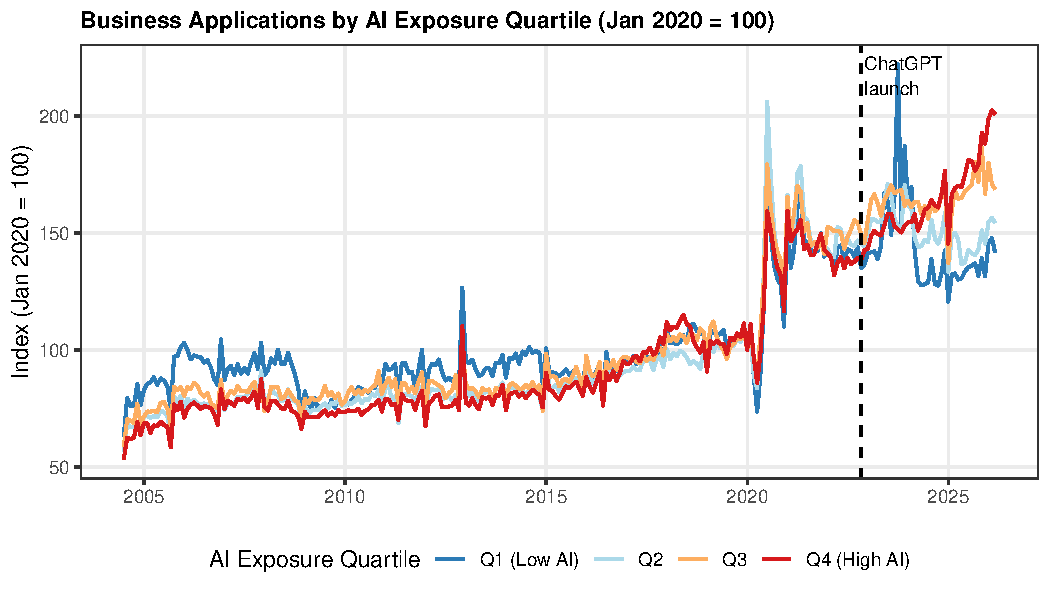
\includegraphics[width=0.85\textwidth]{fig_desc}
  \caption{Business applications by AI exposure quartile (Jan 2020 = 100).
           Dashed vertical lines mark November 2022 (ChatGPT launch) and
           May 2025 (agentic AI tools).}
  \label{fig:desc}
\end{figure}

\subsection{Difference-in-Differences}
\label{sec:results_did}

Table~\ref{tab:did} reports the DiD estimates.
Columns~(1)--(3) pool the entire post-November~2022 period into a single
\textit{Post} indicator; column~(4) splits the post period into a ChatGPT
window (November~2022--April~2025) and an agentic-AI window (May~2025
onwards).
The single-period estimates are attenuated relative to the two-period
specification, consistent with the event-study evidence that the effect
builds gradually and becomes strongest toward the end of the sample.

\begin{table}
\centering
\begin{talltblr}[         %% tabularray outer open
caption={Difference-in-Differences Estimates},
label={tab:did},
note{}={* p \num{< 0.1}, ** p \num{< 0.05}, *** p \num{< 0.01}},
note{ }={Standard errors clustered by 2-digit NAICS sector. Post$_{\text{ChatGPT}}$: Nov 2022 -- Apr 2025. Post$_{\text{Agentic}}$: May 2025 onwards.},
]                     %% tabularray outer close
{                     %% tabularray inner open
width=\linewidth,
colspec={Q[]Q[]Q[]Q[]Q[]},
hline{2}={1-5}{solid, black, 0.05em},
hline{4}={1-5}{solid, black, 0.05em},
hline{1}={1-5}{solid, black, 0.08em},
hline{8}={1-5}{solid, black, 0.08em},
column{2-5}={}{halign=c},
column{1}={}{halign=l},
}                     %% tabularray inner close
& (1) log(BA) & (2) BA Index & (3) BA Level & (4) Two-period \\
Post$_{\text{ChatGPT}}$ $\times$ AI Exposure & \num{0.209} & \num{30.151} & \num{-1607.456} & \num{0.121} \\
& (\num{0.227}) & (\num{30.712}) & (\num{7157.107}) & (\num{0.214}) \\
Observations & \num{4959} & \num{4959} & \num{4959} & \num{4959} \\
R$^2$ & \num{0.982} & \num{0.690} & \num{0.834} & \num{0.983} \\
Sector FE & $\checkmark$ & $\checkmark$ & $\checkmark$ & $\checkmark$ \\
Month FE & $\checkmark$ & $\checkmark$ & $\checkmark$ & $\checkmark$ \\
\end{talltblr}
\end{table}


\subsection{Event Study}
\label{sec:results_es}

Figure~\ref{fig:es} presents the event-study coefficients.
The pre-period estimates ($t < 0$) are small and statistically
indistinguishable from zero, supporting the parallel-trends assumption.
Post-launch, coefficients rise gradually before the 95\,\% confidence
interval clears zero around 2025 ($t \approx +25$ to $+30$), indicating
that the differential effect of AI exposure on business formation became
statistically significant roughly two to three years after the ChatGPT
launch.
This pattern is consistent with a diffusion mechanism: entrepreneurs
require time to learn the tools, identify viable business models, and
translate that into actual EIN filings.
A visible second inflection around $t = +30$ (May~2025, the emergence of
widely available agentic AI tools) suggests a possible amplification of
the initial shock, which the two-period DiD in column~(4) of
Table~\ref{tab:did} is designed to capture.

\begin{figure}[H]
  \centering
  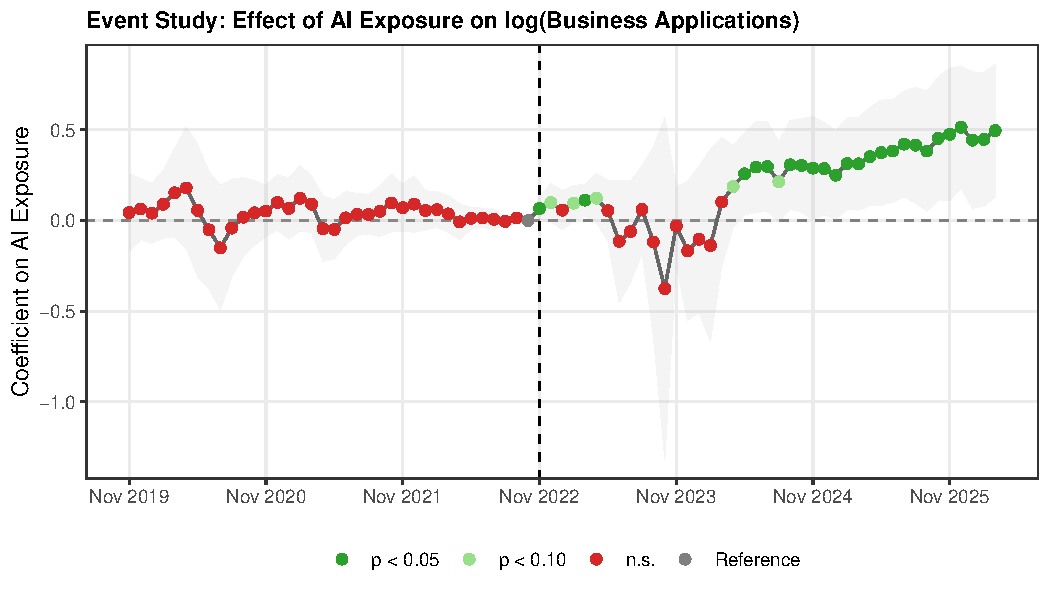
\includegraphics[width=0.85\textwidth]{fig_event_study}
  \caption{Event-study estimates: effect of AI exposure on
           $\log(\text{Business Applications})$ relative to
           November 2022 ($t = 0$). Shaded band is the 95\,\% confidence
           interval based on sector-clustered standard errors.
           The second dashed line marks May 2025 ($t = +30$, agentic AI).}
  \label{fig:es}
\end{figure}

% -----------------------------------------------------------------------
\section{Conclusion}
\label{sec:conclusion}
% -----------------------------------------------------------------------

[Conclusion placeholder.]

% -----------------------------------------------------------------------
\bibliographystyle{plainnat}
\bibliography{references}
% -----------------------------------------------------------------------

\end{document}
